\documentclass{report}
\usepackage{graphicx} % Required for inserting images
\usepackage{geometry}
\usepackage{amsmath}
\usepackage{mathtools}
\usepackage{amssymb}
\usepackage{kotex}
\usepackage{makecell}
\usepackage{bytefield}
\usepackage{listings}
\usepackage{caption}
\usepackage{subcaption}

\captionsetup{labelformat=empty,labelsep=none,font=small}
\lstset{
    basicstyle=\small\ttfamily,
    commentstyle=\small\ttfamily,
    numbers=left,
    columns=flexible,
    breaklines=true,
    captionpos=b,
    xleftmargin=5.0ex,
    aboveskip=1.0em,
}

\title{CSED551 PA\#4 \\[0.5ex] {\normalsize :Camera ISP \& JPEG Development}}
\author{\small{20220848 Minsu Sun}}
\date{\small{December 8, 2024}}

\begin{document}

\maketitle

\section*{Code}

아래는 Camera ISP의 주요 함수인 White Balancing, CFA Interpolation, Gamma Correction에 대한 설명이다.

\begin{lstlisting}[language=Python, caption=awb, firstnumber=15]
def awb(image, cfa_type):
    # Auto White Balance
    height, width = image.shape

    R = []
    G = []
    B = []

    # gather pixels on color filter
    for i in range(height):
        for j in range(width):
            filter = cfa_type[i % 2][j % 2]
            if filter == "R":
                R.append(image[i][j])
            elif filter == "G":
                G.append(image[i][j])
            elif filter == "B":
                B.append(image[i][j])

    # mean values of each color pixels
    R_avg = np.mean(R)
    G_avg = np.mean(G)
    B_avg = np.mean(B)

    # coefficient for auto white balancing
    R_coef = G_avg / R_avg
    B_coef = G_avg / B_avg

    result = image.copy()

    for i in range(height):
        for j in range(width):
            filter = cfa_type[i % 2][j % 2]
            if filter == "R":
                result[i][j] = result[i][j] * R_coef
            elif filter == "B":
                result[i][j] = result[i][j] * B_coef

    return np.clip(result, 0, 1)
\end{lstlisting}

위 코드는 주어진 tiff 이미지를 이용해 auto white balancing을 수행하는 함수이다.
CFA type을 이용해 각 위치의 픽셀이 어떤 color의 데이터인지 판단하고, 이를 이용해 RGB별로 평균 Intensity를 계산한다.
계산한 평균을 이용하여 계수를 결정하고 이를 다시 각 색상별 위치에 곱해 White Balancing을 마무리한다.

\begin{lstlisting}[language=Python, caption=cfa\_interpolation, firstnumber=56]
def cfa_interpolation(image, cfa_type):
    height, width = image.shape
    result = np.zeros((height, width, 3))  # RGB channel

    def get_filter(i, j):
        return cfa_type[i % 2][j % 2]

    def neighbor_mean(i, j, target):
        assert target in ["R", "G", "B"], f"Unkown target: {target}"

        directions = [
            [1, 1], [1, -1], [-1, 1], [-1, -1],
            [1, 0], [0, 1], [-1, 0], [0, -1],
        ]
        neighbor = []

        for direction in directions:
            pos = (i + direction[0], j + direction[1])

            if not (0 <= pos[0] < height and 0 <= pos[1] < width):
                continue

            if target == get_filter(pos[0], pos[1]):
                neighbor.append(image[pos[0]][pos[1]])

        return np.mean(neighbor)

    for i in range(height):
        for j in range(width):
            filter = get_filter(i, j)
            if filter == "R":
                r = image[i][j]
                g = neighbor_mean(i, j, "G")
                b = neighbor_mean(i, j, "B")
            elif filter == "G":
                r = neighbor_mean(i, j, "R")
                g = image[i][j]
                b = neighbor_mean(i, j, "B")
            elif filter == "B":
                r = neighbor_mean(i, j, "R")
                g = neighbor_mean(i, j, "G")
                b = image[i][j]
            result[i][j] = [b, g, r]

    return np.clip(result, 0, 1)
\end{lstlisting}

위 코드는 주어진 tiff 이미지에서 cfa의 배열에 따라 RGB 채널의 이미지를 구성하는 함수이다.
이미지 구성에 사용된 interpolation 방법은 bilinear interpolation이다.
이에 따라 이미지의 각 픽셀 별로 tiff 이미지 상에서의 근처 이웃 센서값을 받아와 이를 평균내어 이미지의 픽셀로 기록한다.
각 위치별로 CFA에 따른 어떤 색에 대한 센서값인지는 \code{get_filter}를 이용하여 계산하고, 주위 이웃의 Intensity 평균은 \code{neighbor_mean}을 통해 계산한다.

\begin{lstlisting}[language=Python, caption=gamma\_correction, firstnumber=118]
def gamma_correction(image, gamma):
    result = image.copy() / 255
    result = result ** (1 / gamma) * 255
    return np.clip(result, 0, 255).astype(np.uint8)
\end{lstlisting}

위 코드는 주어진 이미지에 Gamma Correction을 적용하는 함수이다.
Gamma Correction은 정의에 따라 다음과 같은 식을 이용하여 적용한다.

$$I' = I ^ {\frac{1}{\gamma}}$$

다음은 위에서 제시한 Auto White Balancing, CFA Interpolation,
Gamma Correction 이외에 추가적으로 구현한 ISP Pipeline 모듈을 설명한다.

\begin{lstlisting}[language=Python, caption=sharpening, firstnumber=103]
def sharpening(image, intensity):
    blurred_image = cv2.bilateralFilter(image, 9, 75, 75)
    result = image.copy()
    result = image + intensity * (image - blurred_image)
    return np.clip(result, 0, 255).astype(np.uint8)
\end{lstlisting}

위는 주어진 이미지를 Sharpening하는 함수로, OpenCV의 `bilateralFilter'를 이용해 lowpass filter가 적용된 이미지를 생성하였다.
이후 이를 sharpening을 진행하는 순서에 따라 주어진 intensity가 적용된 sharpened 이미지를 반환한다.

\begin{lstlisting}[language=Python, caption=saturation, firstnumber=111]
def saturation(image, intensity):
    image_HSV = cv2.cvtColor(image, cv2.COLOR_BGR2HSV)
    delta = np.full(image.shape, (0, intensity, 0), dtype=np.uint8)
    result = np.add(image_HSV, delta).astype(np.uint8)
    return cv2.cvtColor(np.clip(result, 0, 255), cv2.COLOR_HSV2BGR)
\end{lstlisting}

위는 주어진 이미지의 채도를 올려주는 함수이다.
주어진 이미지를 기본 RGB 색역에서 HSV 색역으로 변환 후, S(aturation) 채널에 주어진 intensity만큼 증가치를 더해 채도를 증가시킨다.
이후 다시 RGB 색역으로 되돌려 반환한다.

\begin{lstlisting}[language=Python, caption=color\_temp, firstnumber=135]
def color_temp(image, target_temp):
    kelvin_table = {
        1000: (255, 56, 0),
        1500: (255, 109, 0),
        2000: (255, 137, 18),
        2500: (255, 161, 72),
        3000: (255, 180, 107),
        3500: (255, 196, 137),
        4000: (255, 209, 163),
        4500: (255, 219, 186),
        5000: (255, 228, 206),
        5500: (255, 236, 224),
        6000: (255, 243, 239),
        6500: (255, 249, 253),
        7000: (245, 243, 255),
        7500: (235, 238, 255),
        8000: (227, 233, 255),
        8500: (220, 229, 255),
        9000: (214, 225, 255),
        9500: (208, 222, 255),
        10000: (204, 219, 255)}
    r, g, b = kelvin_table[target_temp]
    matrix = np.array([
        [b / 255, 0, 0],
        [0, g / 255, 0],
        [0, 0, r / 255]
    ])
    result = np.matmul(image, matrix)
    return np.clip(result, 0, 255).astype(np.uint8)
\end{lstlisting}

위 함수는 주어진 타겟 색온도로의 색 보정을 진행하는 함수이다.
주어진 \code{kelvin_table}에서 타겟 색온도의 R, G, B 정보를
가져와 이를 토대로 Color Correction Matrix를 만들고, 이를
이미지에 적용하여 색보정을 진행한다.

\section*{Discussion - Step by Step}

\subsection*{AWB \& CFA Interpolation}

\begin{figure}[htbp]
    \centering

    \subfloat[After AWB \& CFA Interpolation]{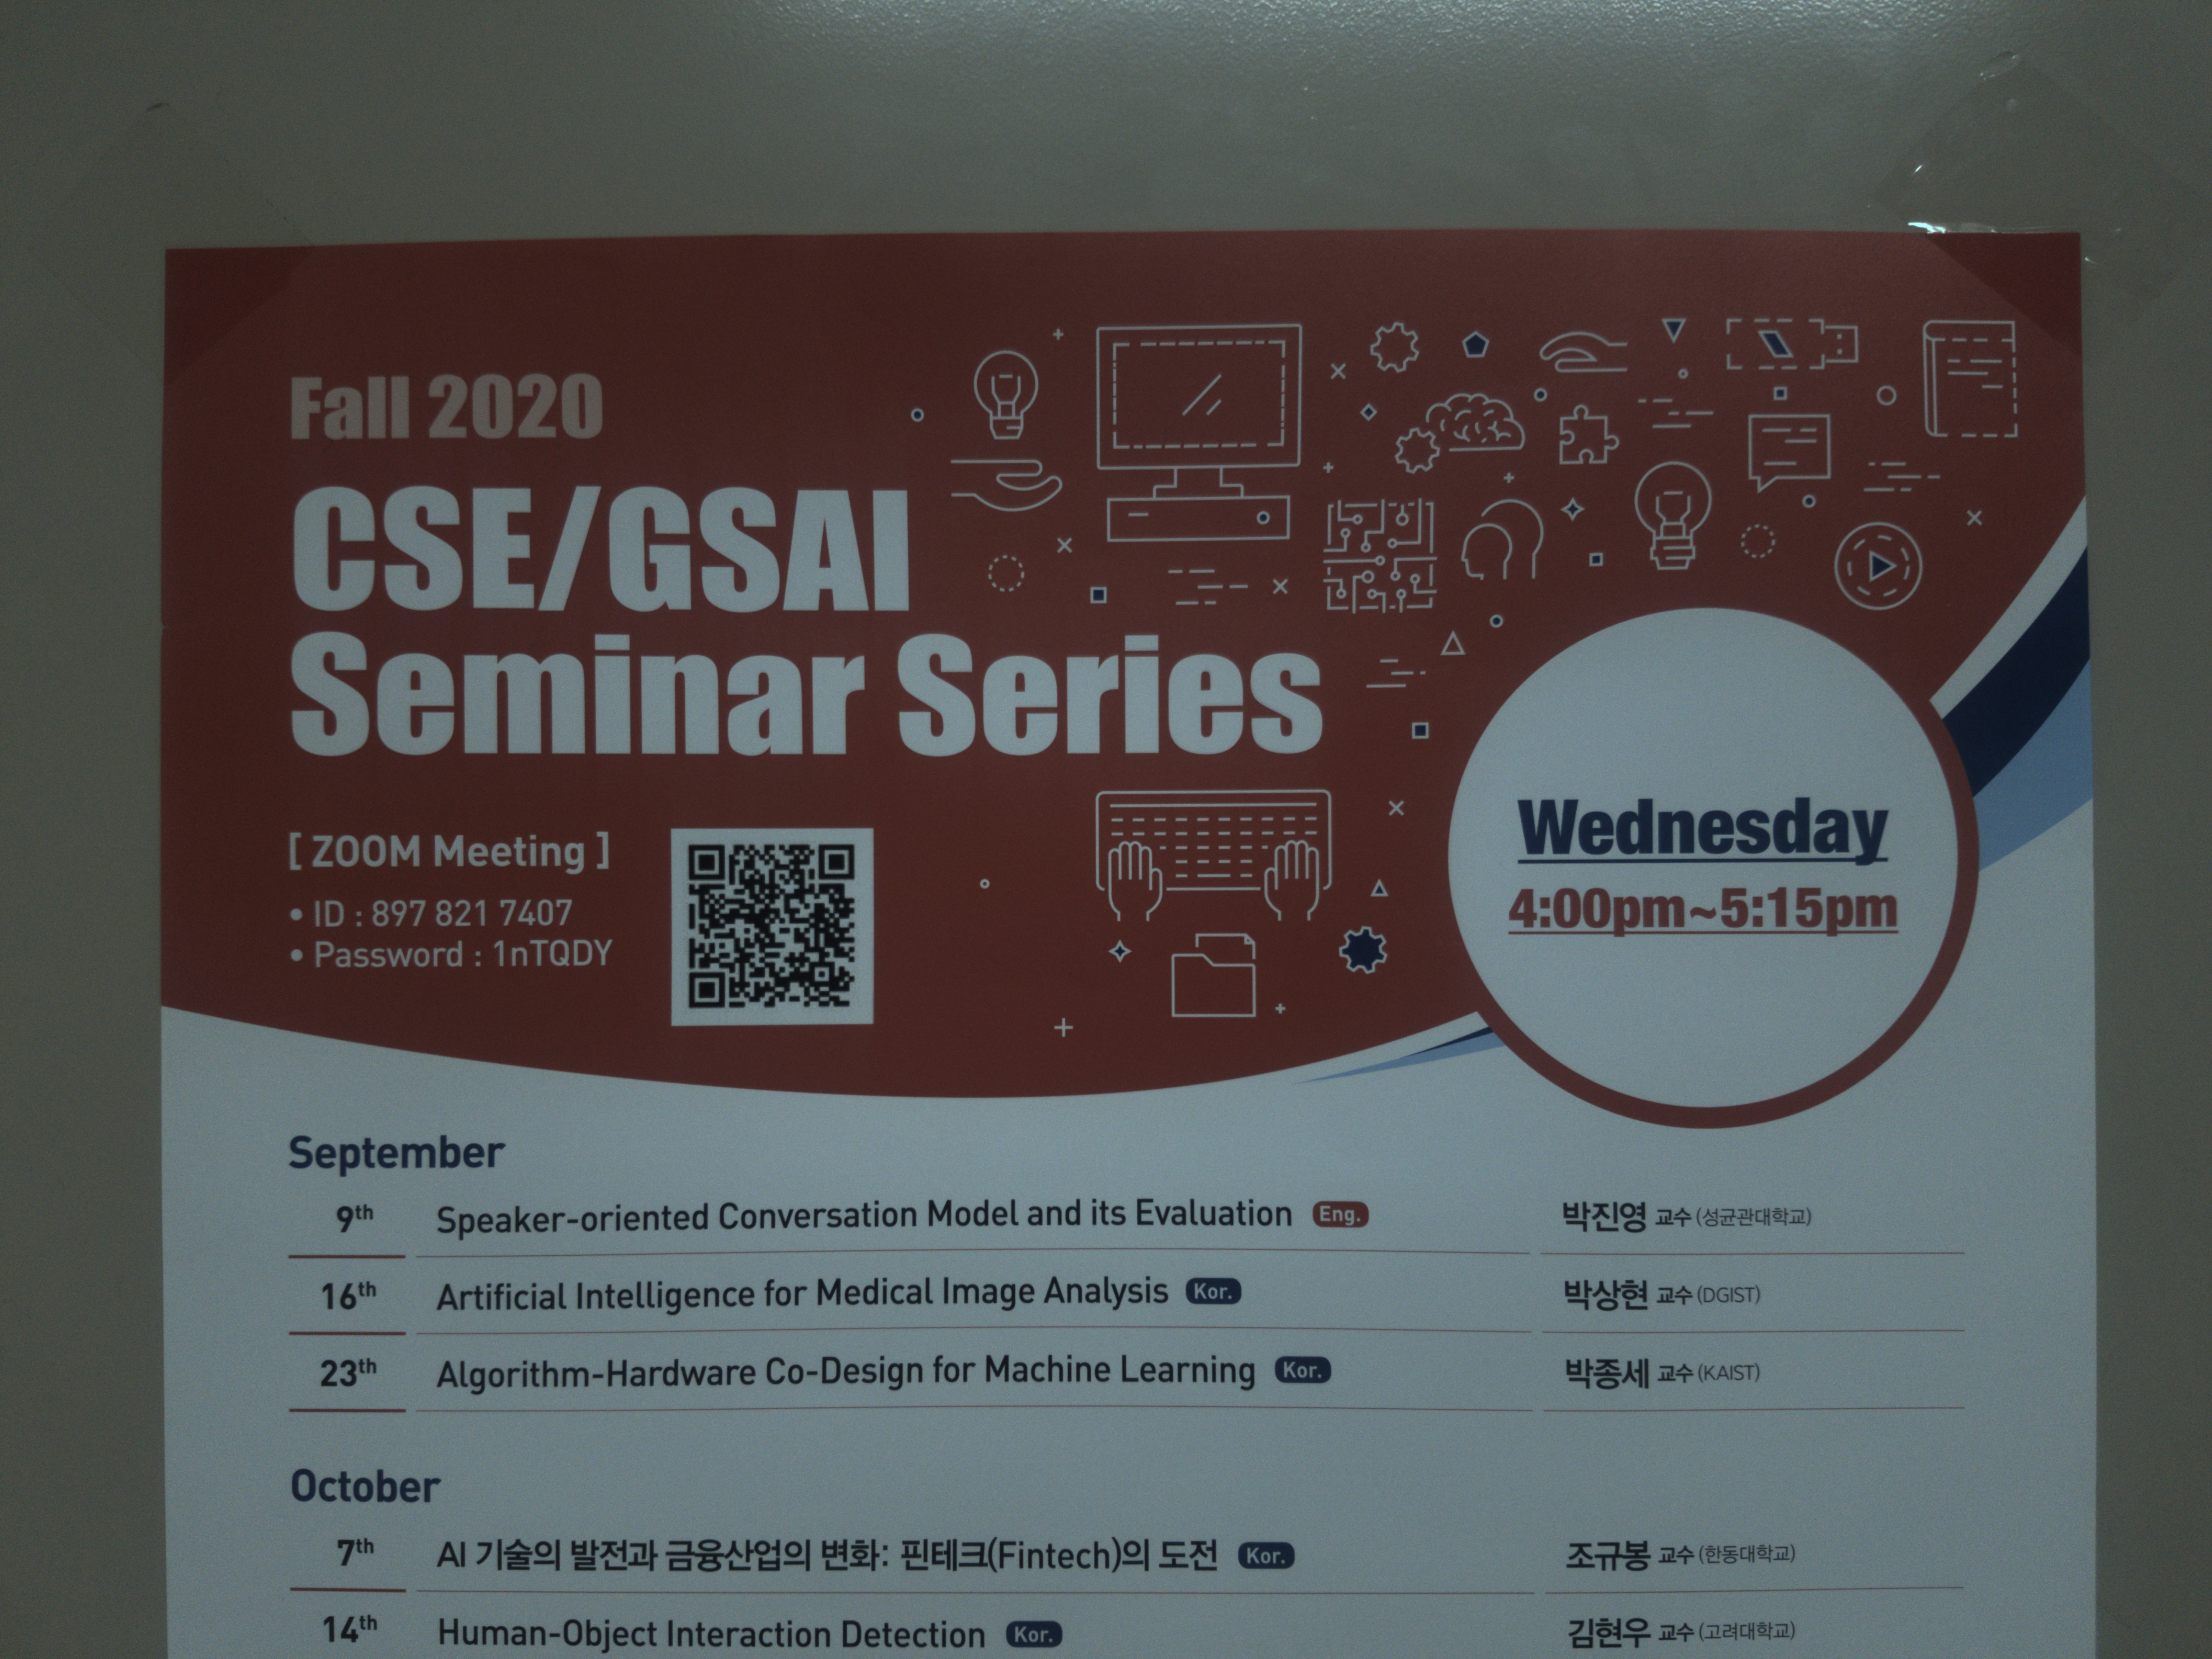
\includegraphics[width=0.6\linewidth]{../images/result/20200917_170752_aux_0.jpg}}

    \caption{Discussion}
\end{figure}

위는 .tiff 파일에서 Auto White Balancing과 CFA Interpolation을 완료한 이미지이다.

\subsection*{Sharpening}

\begin{figure}[htbp]
    \centering

    \subfloat[After Sharpening]{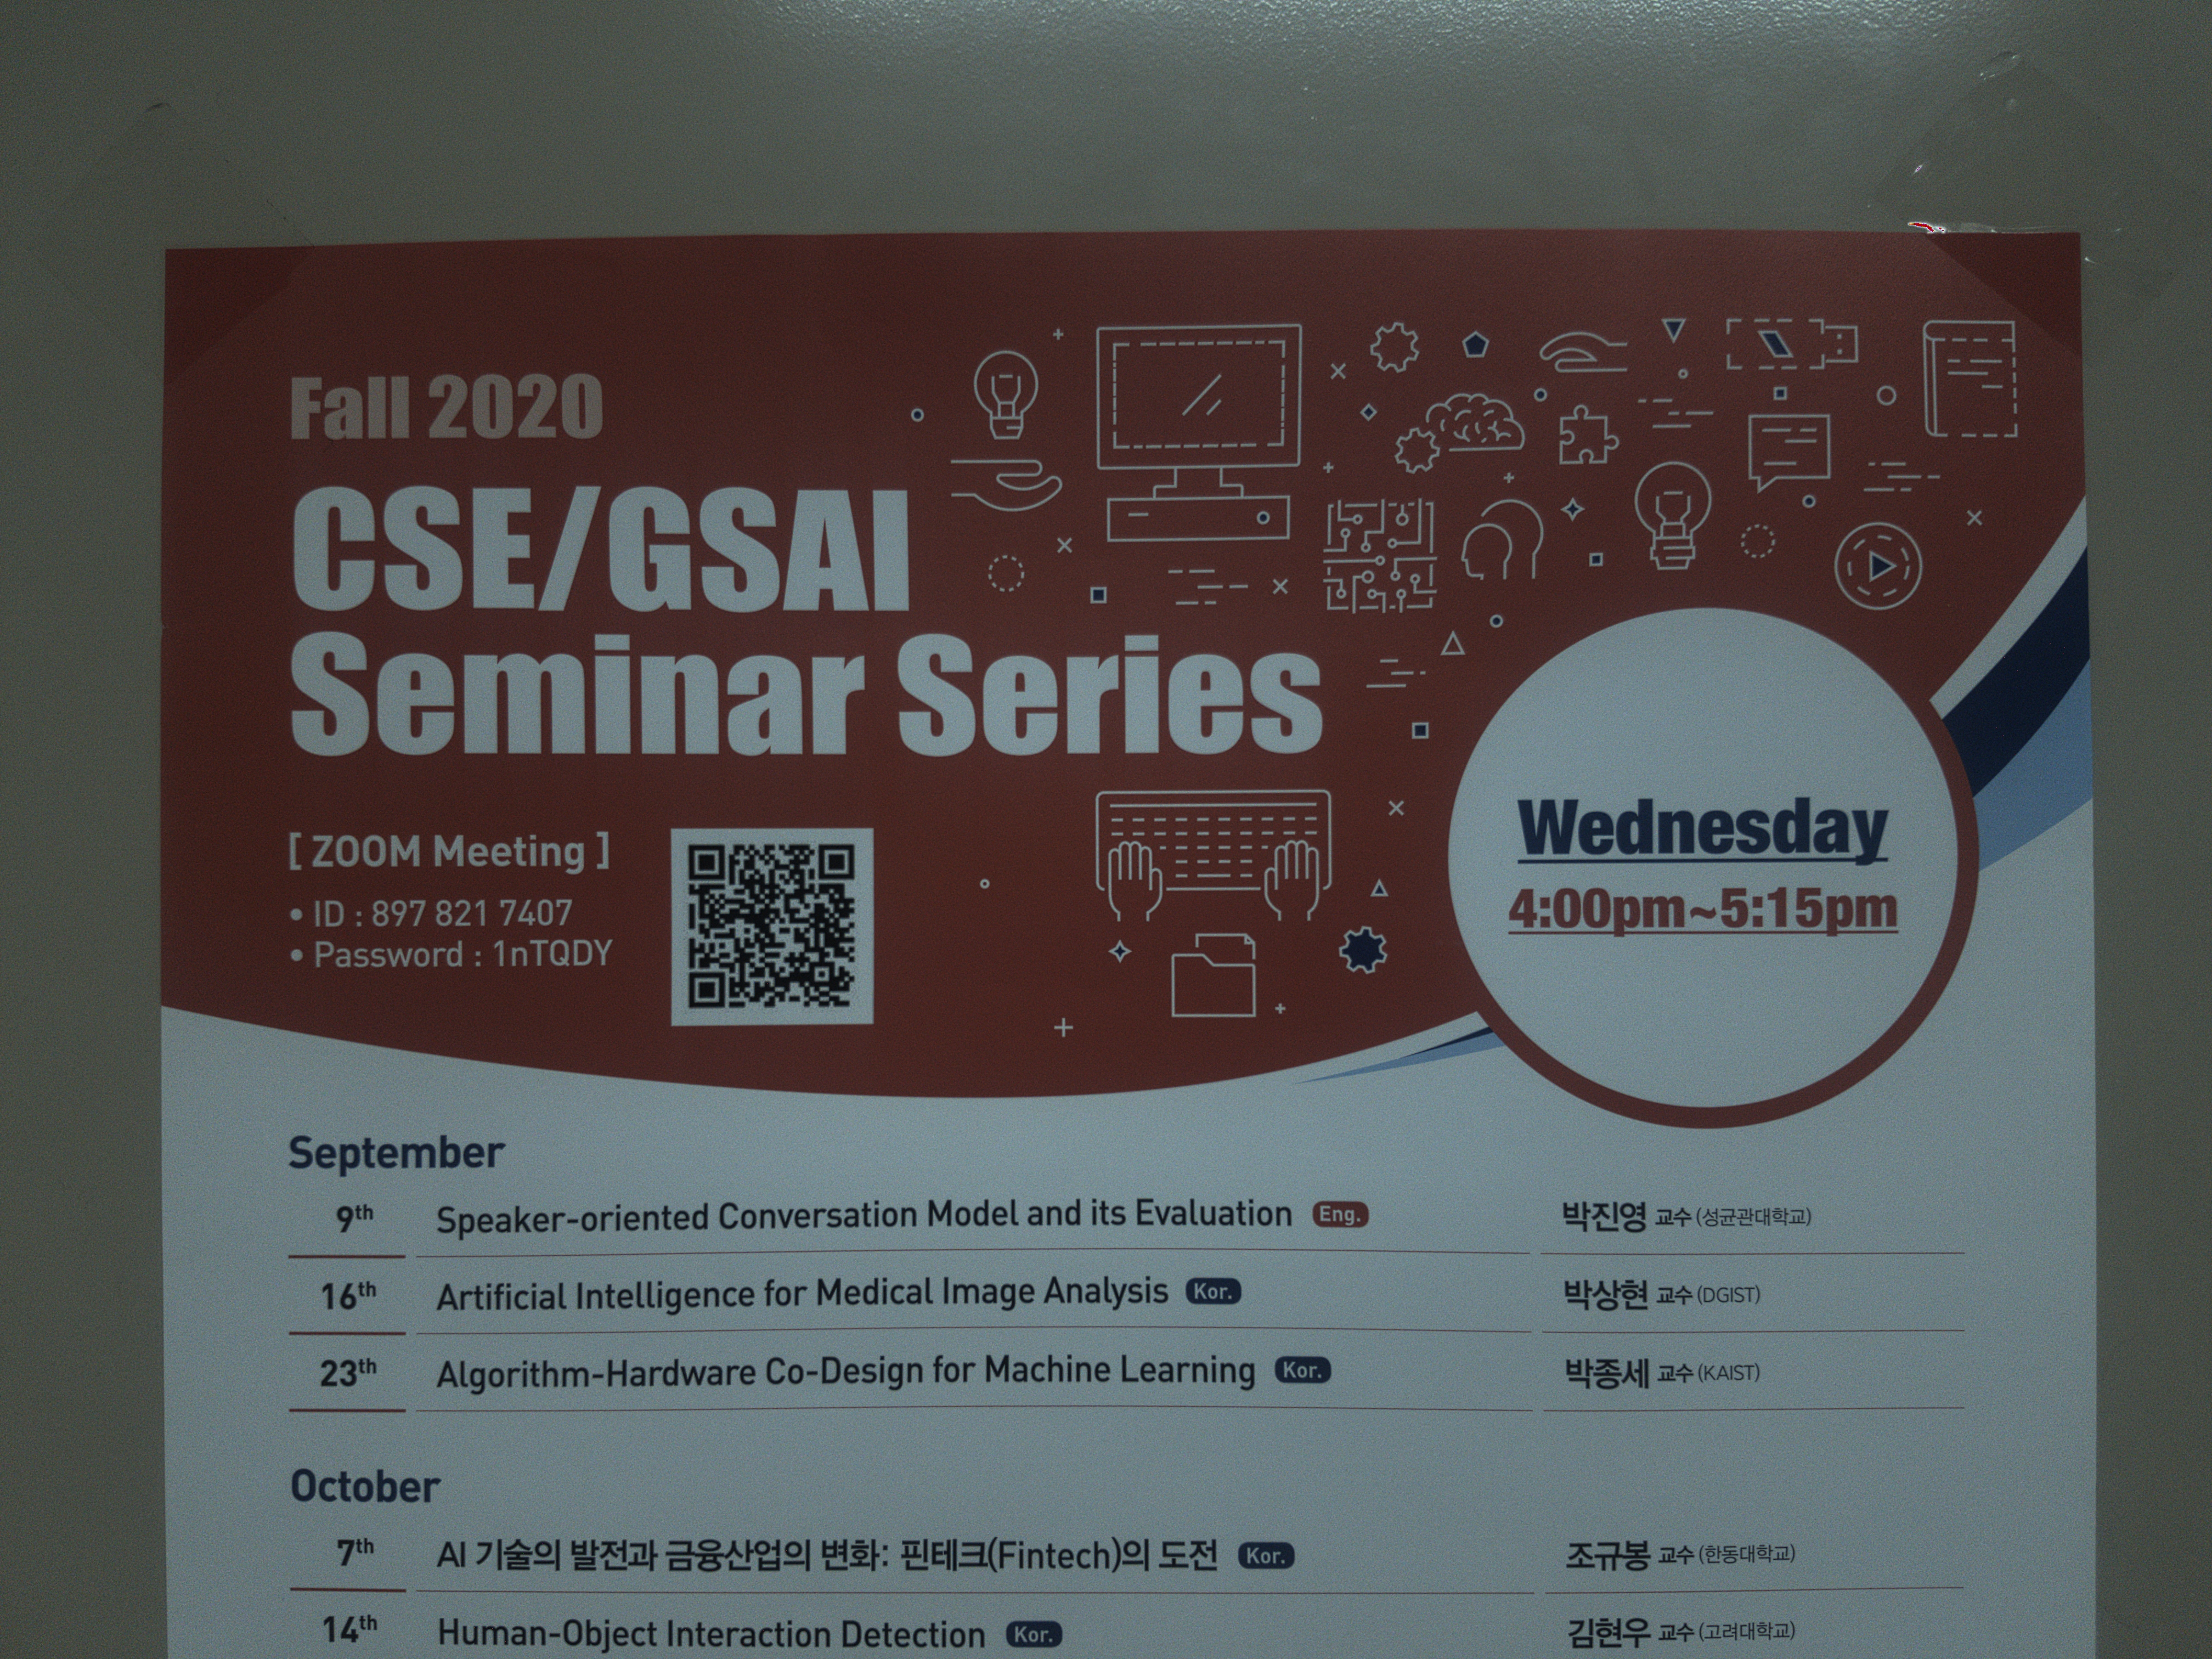
\includegraphics[width=0.6\linewidth]{../images/result/20200917_170752_aux_1.jpg}}

    \caption{Discussion}
\end{figure}

위는 이후 Sharpening\(\alpha = 1\)을 적용한 이미지이다.
크게 차이가 없어보이지만 세밀한 디테일들이 살아난 것을 확인할 수 있다.

\subsection*{Saturation}

\begin{figure}[htbp]
    \centering

    \subfloat[After Saturation]{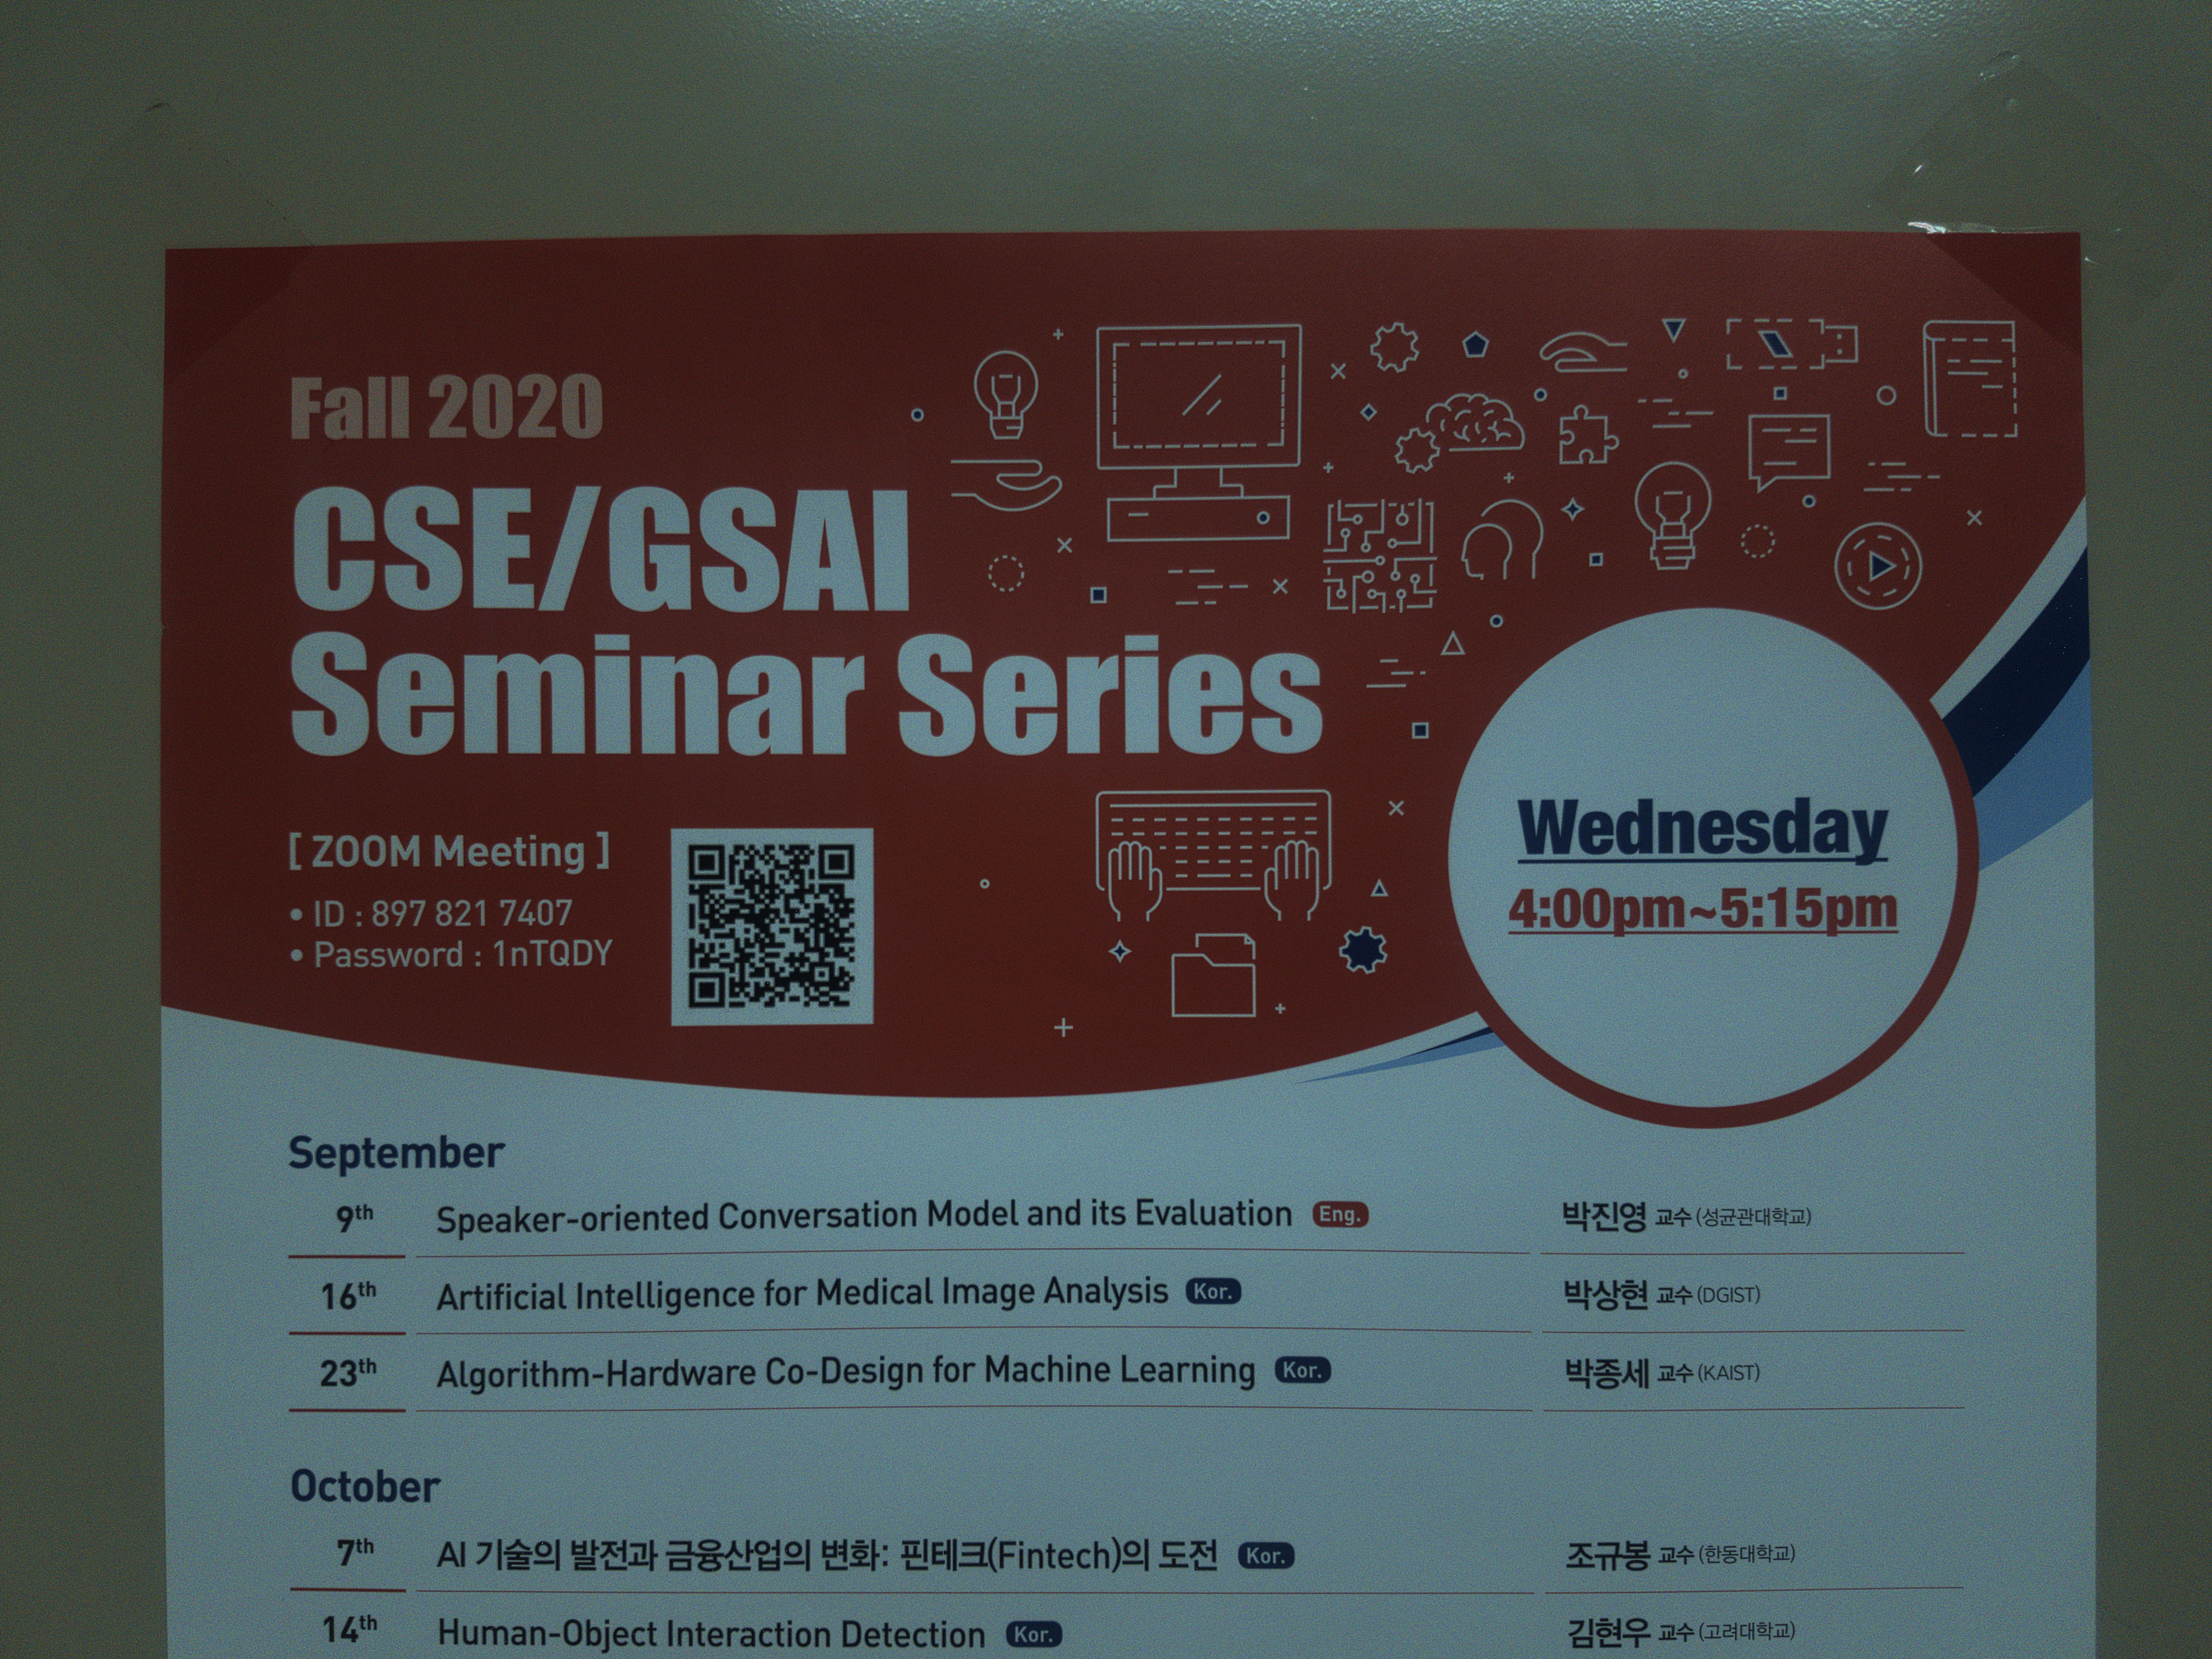
\includegraphics[width=0.6\linewidth]{../images/result/20200917_170752_aux_2.jpg}}

    \caption{Discussion}
\end{figure}

위는 이후 Saturation\(\alpha = 30\)을 적용한 이미지이다.
어두운 톤에 의해 크게 부각되지는 않지만 톤이 올라간 결과를 확인할 수 있다.

\subsection*{Gamma Correction}

\begin{figure}[htbp]
    \centering

    \subfloat[After Gamma Correction]{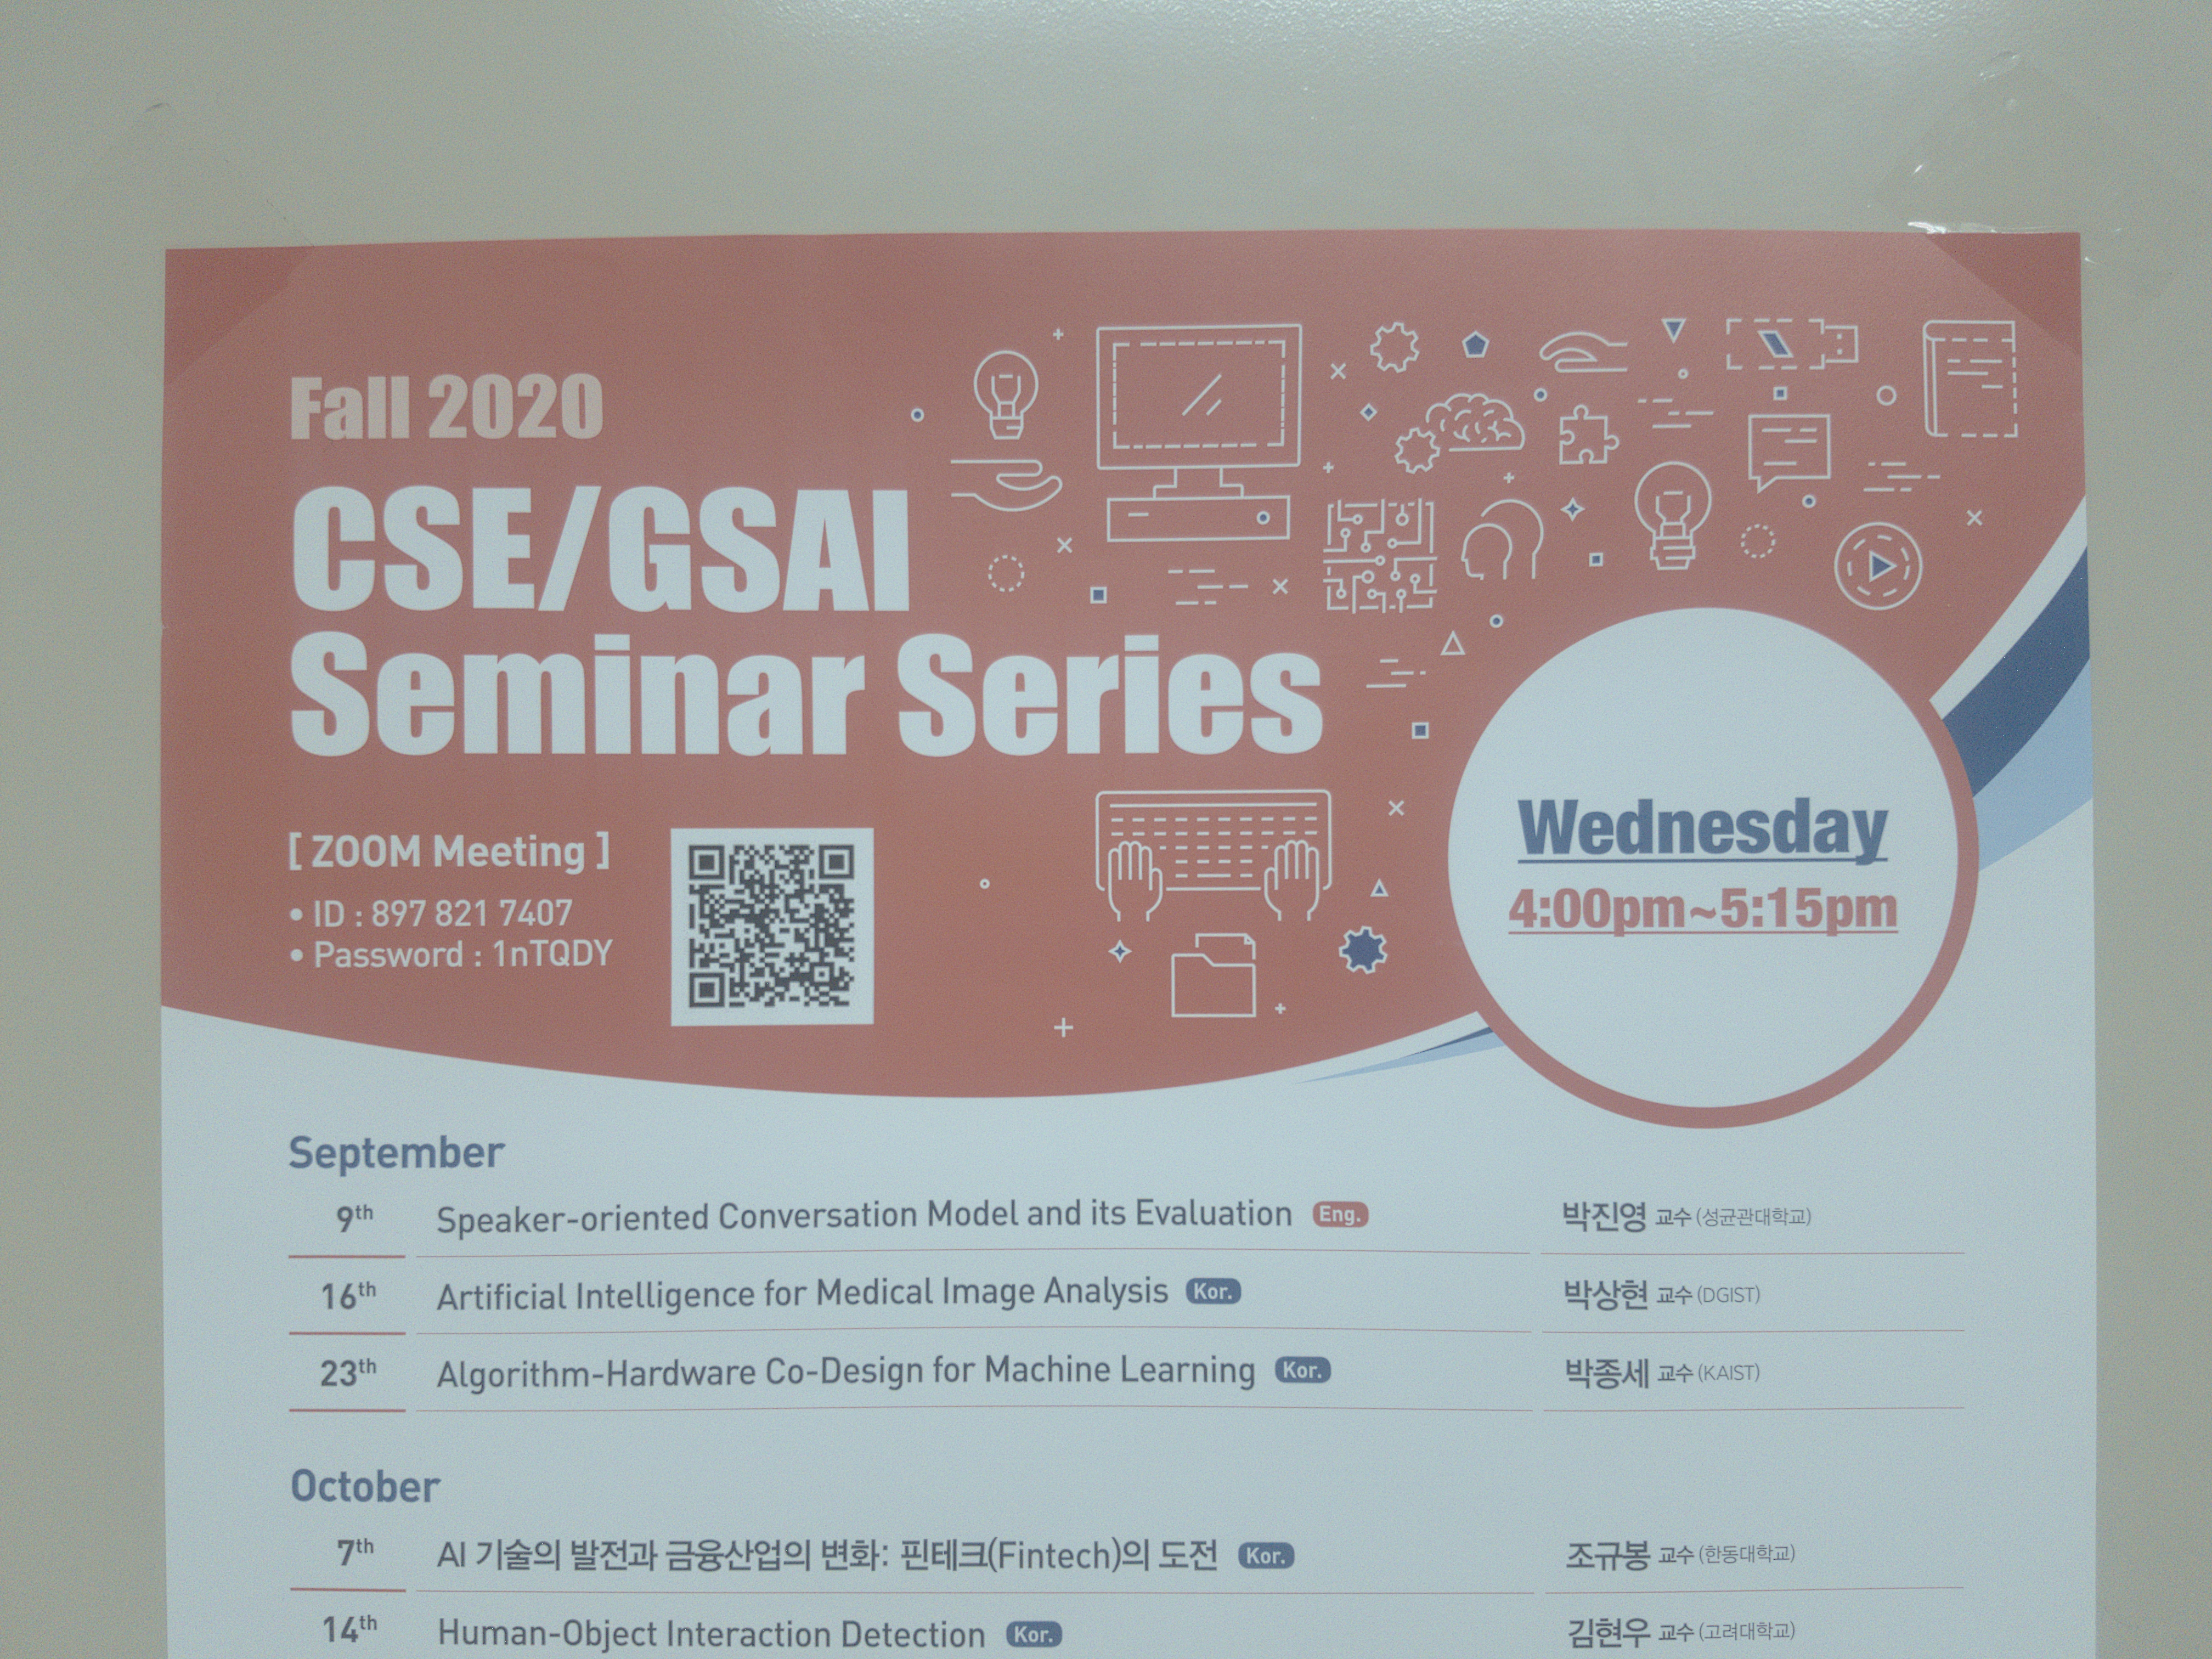
\includegraphics[width=0.6\linewidth]{../images/result/20200917_170752_aux_3.jpg}}

    \caption{Discussion}
\end{figure}

위는 이후 Gamma Correction\(\gamma = 2.4\) 적용한 이미지이다.
기존의 어두운 톤이 사라지고 밝아진 것을 확인할 수 있다.

\subsection*{Color Correction(Color Temperature)}

\begin{figure}[htbp]
    \centering

    \subfloat[After Color Correction]{\includegraphics[width=0.6\linewidth]{../images/result/20200917_170752.jpg}}

    \caption{Discussion}
\end{figure}

위는 이후 Color Correction\(Color Temperature = 5500K\)을 적용한 이미지이다.
이전 단계 대비 너무 밝은 부분이 어느 정도 제어된 결과를 확인할 수 있다.

\section*{Discussion - Result}

\begin{figure}[htbp]
    \centering

    \subfloat[After ISP]{\includegraphics[width=0.3\linewidth]{../images/result/20200917_170752.jpg}}
    \hspace{1pt}
    \subfloat[Result from Samsung]{\includegraphics[width=0.3\linewidth]{../images/20200917_170752.jpg}}

    \caption{Discussion}
\end{figure}

위는 Camera ISP Pipeline의 최종 결과물과 Samsung의 ISP 결과이다.
삼성의 ISP 결과와는 달리 노랑색의 톤을 띄며, 이미지의 대비가 떨어지는 듯한 결과를 보인다.

\end{document}
